\chapter{Technology and Paper Overview}
\setcounter{equation}{0}
\section{Selected Paper}
M. Misiek and T. Hyla, ``XGBoost-Based URL Phishing Detection Method With Cross-Dataset Validation,'' \textit{IEEE Access}, vol. 14, 2026, pp. 43200--43212, doi: 10.1109/ACCESS.2026.3672690. The article was published online on 10 March 2026.\cite{bib1}

\section{Objectives}
\begin{itemize}
\item Develop an XGBoost-based method to classify potentially malicious URLs.
\item Evaluate the model on datasets from different sources rather than relying on a single split.
\item Identify URL features that provide useful and stable signals across datasets.
\item Tune the model using Bayesian hyperparameter optimisation.
\item Compare detection metrics and computational characteristics with a neural network and baseline classifiers.
\item Describe a browser plug-in workflow that labels URLs as safe, suspicious, or potentially harmful.
\end{itemize}

\section{Datasets}
The authors use three datasets. The custom dataset contains 75,738 URLs assembled from PhishTank, AdaURL, the Kaggle Phishing URLs Dataset by Hassaan Mustafavi, and PhishDataset. GramBeddings contains 639,723 URLs and is used for feature analysis and cross-dataset evaluation. PhiUSIIL provides an independent evaluation set; the feature-compatible subset used in the experiments contains 47,103 URLs. These datasets differ in scale and URL characteristics, which makes them useful for studying generalisation.\cite{bib1}

\section{Proposed Pipeline}
The high-level pipeline is: URL input; allowlist/blocklist lookup; extraction of more than 90 candidate features; cross-dataset analysis and selection of eight stable features; Bayesian hyperparameter optimisation; XGBoost prediction; risk classification; and display of the result in a browser extension. Users may also confirm classifications, allowing domains to be added to the relevant allowlist or blocklist.\cite{bib1}

\begin{figure}[htbp]
\centering
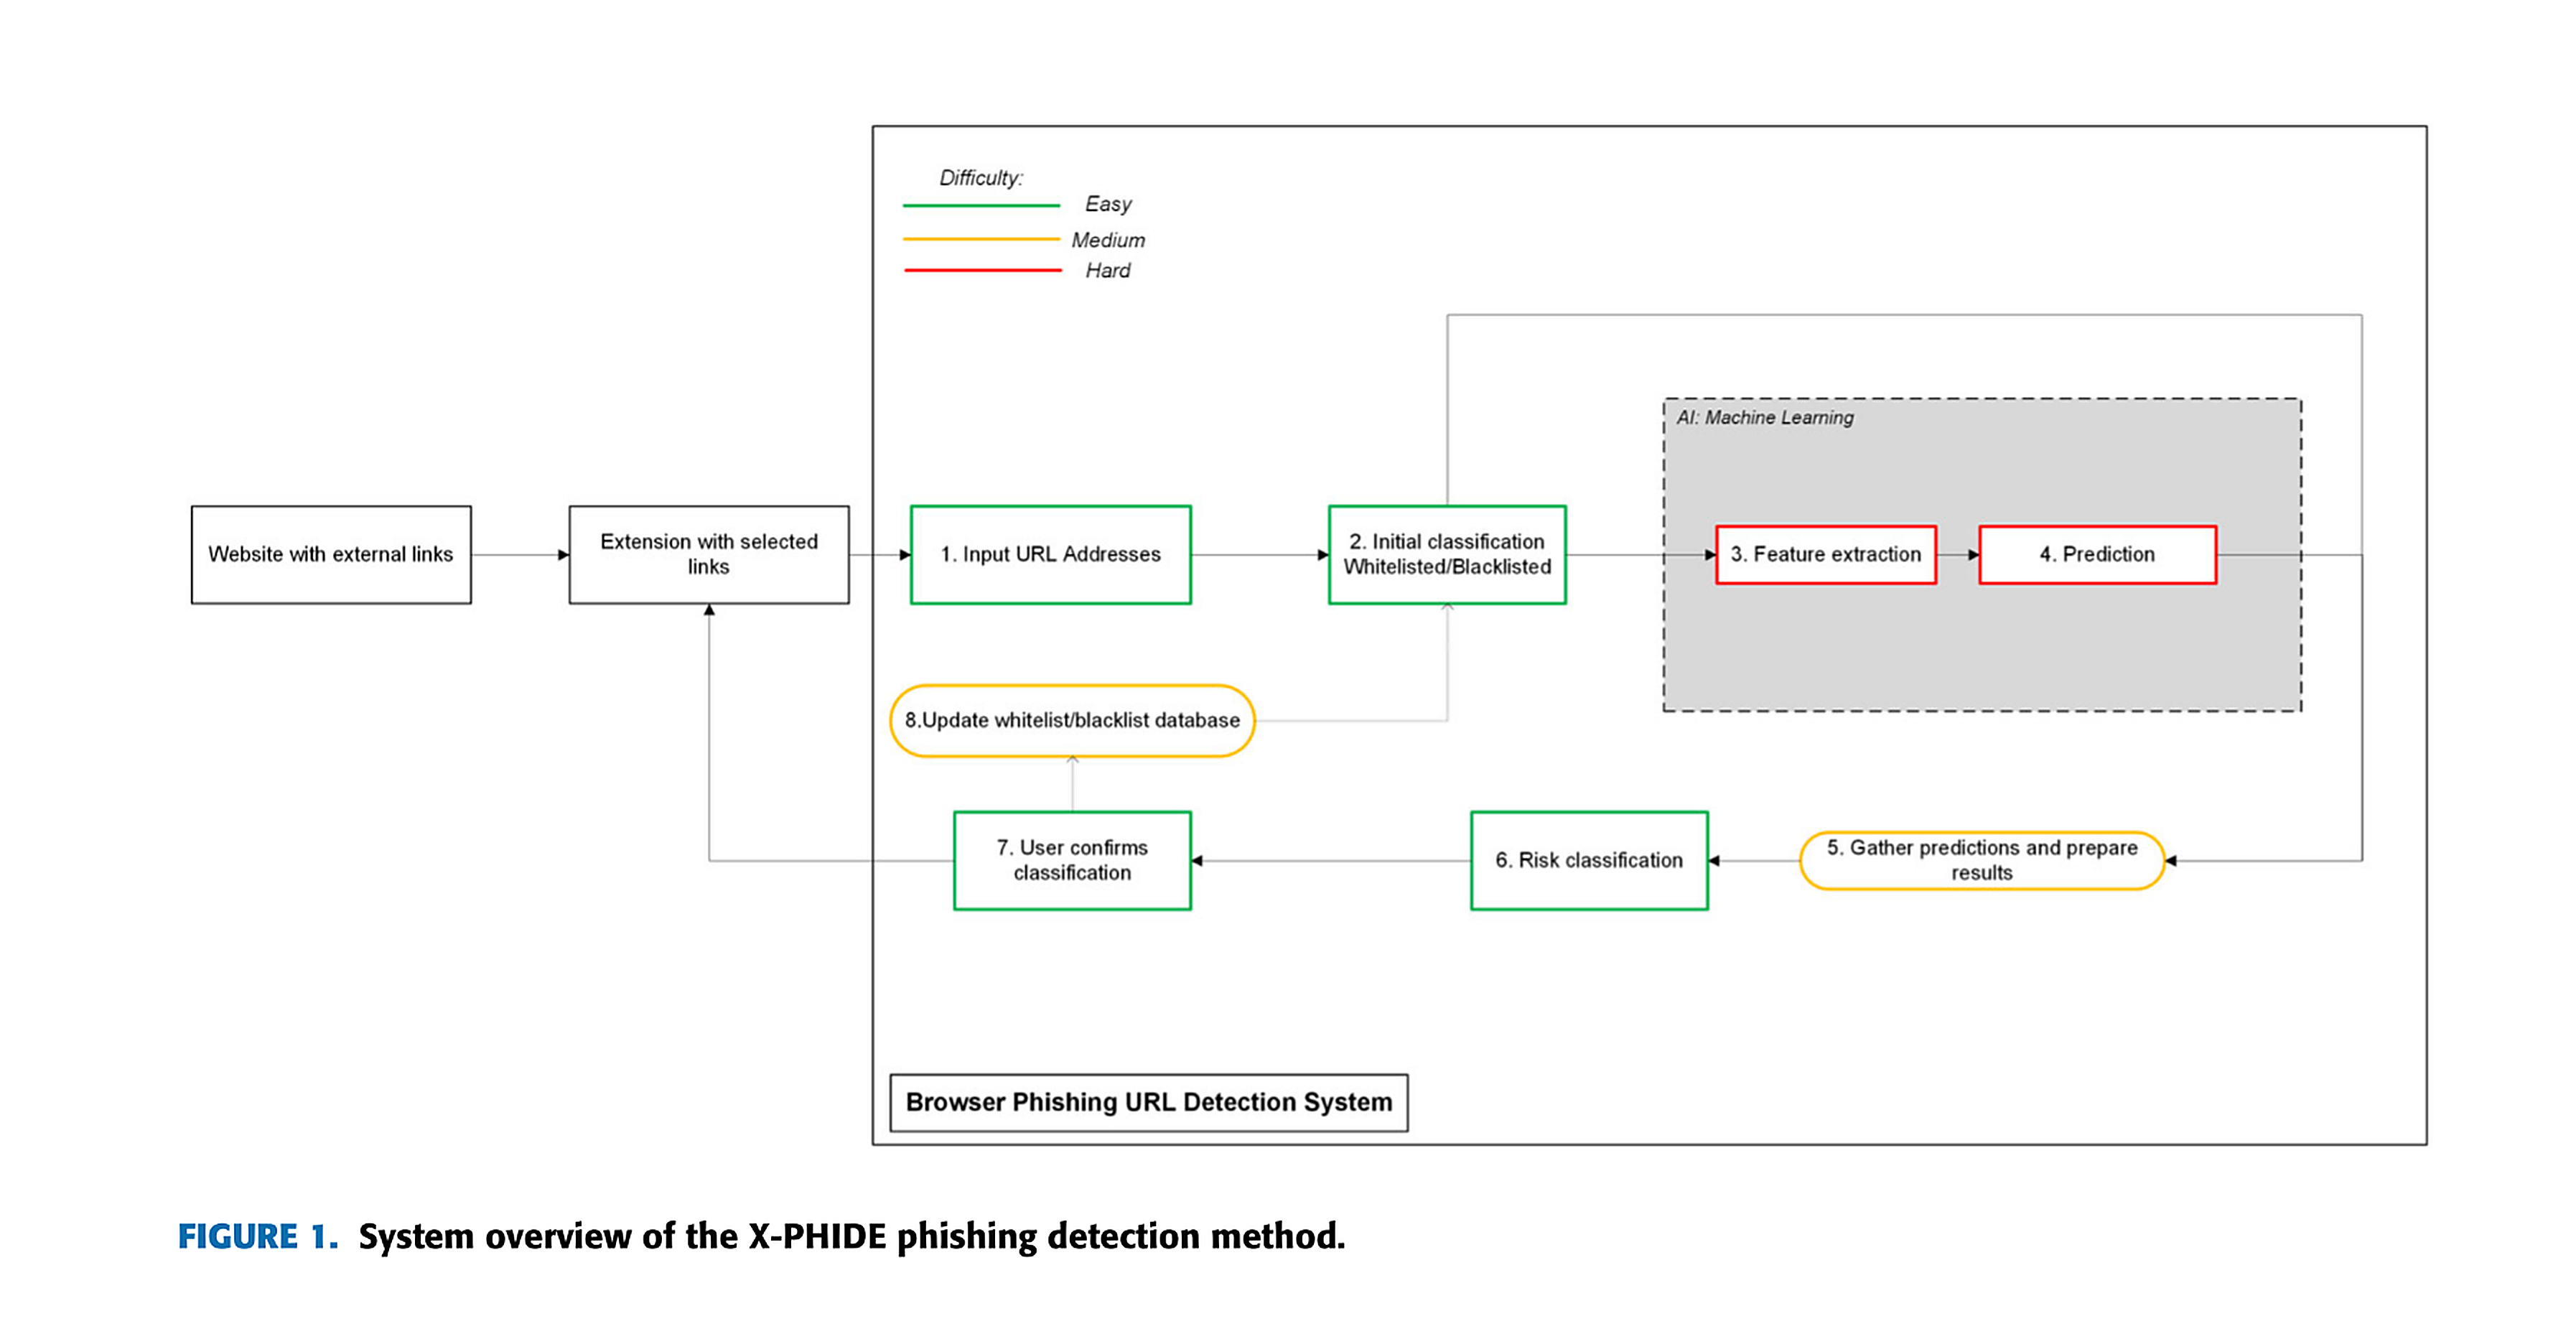
\includegraphics[width=\textwidth,keepaspectratio]{images/systemOverview.png}
\caption{System overview of the browser-based X-PHIDE phishing detection method.}
\label{fig:system-overview}
\end{figure}

\section{Main Contributions}
The main contribution is the evaluation of URL phishing detection under dataset shift. The paper also examines feature-importance stability, reports dataset-specific results and thresholds, and compares XGBoost with a neural network in terms of accuracy, training time, inference time, and memory use.
